% Choose one to switch between slides and handout
\documentclass[]{beamer}
%\documentclass[handout]{beamer}

% Video Meta Data
\title{Smart Contracts and Decentralized Finance Applications}
\subtitle{Public Blockchain Primer}
\author{Prof. Dr. Fabian Schär}
\institute{University of Basel}

% Config File
% Packages
\usepackage[utf8]{inputenc}
\usepackage{hyperref}
\usepackage{gitinfo2}
\usepackage{tikz}
 \usetikzlibrary{calc}
\usepackage{amsmath}
\usepackage{mathtools}
\usepackage{bibentry}
\usepackage{xcolor}
\usepackage{colortbl} % Add colour to LaTeX tables
\usepackage{caption}
\usepackage[export]{adjustbox}
\usepackage{pgfplots} \pgfplotsset{compat = 1.17}
\usepackage{makecell}
\usepackage{fancybox}
\usepackage{ragged2e}
\usepackage{fontawesome}
\usepackage{seqsplit}
\usepackage{tabularx}
\usepackage{tcolorbox}
\usepackage{booktabs} % use instead  \hline in tables

% Color Options
\definecolor{highlight}{rgb}{0.65,0.84,0.82}
\definecolor{focus}{rgb}{0.72, 0, 0}
\definecolor{lightred}{rgb}{0.8,0.5,0.5}
\definecolor{midgray}{RGB}{190,195,200}

 %UniBas Main Colors
\definecolor{mint}{RGB}{165,215,210}
\definecolor{anthracite}{RGB}{45,55,60}
\definecolor{red}{RGB}{210,5,55}

 %UniBas Color Palette (for graphics)
\definecolor{strongmint}{RGB}{30,165,165}
\definecolor{darkmint}{RGB}{0,110,110}
\definecolor{softanthracite}{RGB}{140,145,150}
\definecolor{brightanthracite}{RGB}{190,195,200}
\definecolor{softred}{RGB}{235,130,155}

%Custom Colors
\definecolor{lightergray}{RGB}{230, 230, 230}



% Beamer Template Options
\beamertemplatenavigationsymbolsempty
\setbeamertemplate{footline}[frame number]
\setbeamercolor{structure}{fg=black}
\setbeamercolor{footline}{fg=black}
\setbeamercolor{title}{fg=black}
\setbeamercolor{frametitle}{fg=black}
\setbeamercolor{item}{fg=black}
\setbeamercolor{}{fg=black}
\setbeamercolor{bibliography item}{fg=black}
\setbeamercolor*{bibliography entry title}{fg=black}
\setbeamercolor{alerted text}{fg=focus}
\setbeamertemplate{items}[square]
\setbeamertemplate{enumerate items}[default]
\captionsetup[figure]{labelfont={color=black},font={color=black}}
\captionsetup[table]{labelfont={color=black},font={color=black}}

\setbeamertemplate{bibliography item}{\insertbiblabel}

%tcolor boxes
\newtcolorbox{samplecode}[2][]{
  colback=mint, colframe=darkmint, coltitle=white,
  fontupper = \ttfamily\scriptsize, fonttitle= \bfseries\scriptsize,
  boxrule = 0mm, arc = 0mm,
  boxsep = 1.3mm, left = 0mm, right = 0mm, top = 0.5mm, bottom = 0mm, middle=0mm,
  #1,title=#2}
  
\newtcolorbox{keytakeaway}[2][]{
  colback=softred, colframe=red, coltitle=white,
  fontupper = \scriptsize, fonttitle= \bfseries\scriptsize,
  boxrule = 0mm, arc = 0mm,
  boxsep = 1.3mm, left = 0mm, right = 0mm, top = 0.5mm, bottom = 0mm, middle=0mm,
  #1,title=#2}

\newtcolorbox{exercise}[2][]{
  colback=brightanthracite, colframe=anthracite, coltitle=white,
  fontupper = \scriptsize, fonttitle= \bfseries\scriptsize,
  boxrule = 0mm, arc = 0mm,
  boxsep = 1.3mm, left = 0mm, right = 0mm, top = 0.5mm, bottom = 0mm, middle=0mm,
  #1,title=#2}



% Link Icon Command 
\newcommand{\link}{%
    \tikz[x=1.2ex, y=1.2ex, baseline=-0.05ex]{%
        \begin{scope}[x=1ex, y=1ex]
            \clip (-0.1,-0.1)
                --++ (-0, 1.2)
                --++ (0.6, 0)
                --++ (0, -0.6)
                --++ (0.6, 0)
                --++ (0, -1);
            \path[draw,
                line width = 0.5,
                rounded corners=0.5]
                (0,0) rectangle (1,1);
        \end{scope}
        \path[draw, line width = 0.5] (0.5, 0.5)
            -- (1, 1);
        \path[draw, line width = 0.5] (0.6, 1)
            -- (1, 1) -- (1, 0.6);
        }
    }

% Other commands
\newcommand\tab[1][0.5cm]{\hspace*{#1}} % for code boxes


% Read Git Data from Github Actions Workflow
% Defaults to gitinfo2 for local builds
\IfFileExists{gitInfo.txt}
	{\input{gitInfo.txt}}
	{
		\newcommand{\gitRelease}{(Local Release)}
		\newcommand{\gitSHA}{\gitHash}
		\newcommand{\gitDate}{\gitAuthorIsoDate}
	}

% Custom Titlepage
\defbeamertemplate*{title page}{customized}[1][]
{
  \vspace{-0cm}\hfill\includegraphics[width=2.5cm]{../config/logo_cif}
  \includegraphics[width=1.9cm]{../config/seal_wwz}
  \\ \vspace{2em}
  \usebeamerfont{title}\textbf{\inserttitle}\par
  \usebeamerfont{title}\usebeamercolor[fg]{title}\insertsubtitle\par  \vspace{1.5em}
  \small\usebeamerfont{author}\insertauthor\par
  \usebeamerfont{author}\insertinstitute\par \vspace{2em}
  \usebeamercolor[fg]{titlegraphic}\inserttitlegraphic
    \tiny \noindent \texttt{Release Ver.: \gitRelease}\\ 
    \texttt{Version Hash: \gitSHA}\\
    \texttt{Version Date: \gitDate}\\ \vspace{1em}
    
    
    \iffalse
  \link \href{https://github.com/cifunibas/Bitcoin-Blockchain-Cryptoassets/blob/main/slides/intro.pdf}
  {Get most recent version}\\
  \link \href{https://github.com/cifunibas/Bitcoin-Blockchain-Cryptoassets/blob/main/slides/intro.pdf}
  {Watch video lecture}\\ 
  
  \fi
  
  \vspace{1em}
  License: \texttt{Creative Commons Attribution-NonCommercial-ShareAlike 4.0 International}\\\vspace{2em}
  \includegraphics[width = 1.2cm]{../config/license}
}


% tikzlibraries
\usetikzlibrary{decorations.pathreplacing}
\usetikzlibrary{decorations.markings}
\usetikzlibrary{positioning}
\usetikzlibrary{calc}
\captionsetup{font=footnotesize}

%%%%%%%%%%%%%%%%%%%%%%%%%%%%%%%%%%%%%%%%%%%%%%
%%%%%%%%%%%%%%%%%%%%%%%%%%%%%%%%%%%%%%%%%%%%%%
\begin{document}

\thispagestyle{empty}
\begin{frame}[noframenumbering]
	\titlepage
\end{frame}

%%% TODO: bib ref of Bitcoin whitepaper
\begin{frame}{Blockchain Origin}

\centering
\includegraphics[width = 5cm, frame]{../assets/images/nakamoto_cover}
		
\textbf{Bitcoin: A Peer-to-Peer Electronic Cash System} \\ 
Satoshi Nakamoto \\
\href{https://bitcoin.org/bitcoin.pdf}{\link Online version}

\end{frame}
%%%

%%% TODO: maybe link to Bitcoin primer video where "malicious" centralized third parties are addressed
\begin{frame}{Recap: Bitcoin as a New Asset Class}
Bitcoin enables the exchange of monetary units \textcolor{focus}{without the need for a centralized third party}. The underlying technology solves three problems of distributed ledgers which operate on a global scale:

\begin{itemize}
\item \textbf{Transaction capacity:} anyone can initiate transactions.
\item \textbf{Transaction legitimacy:} the authenticity and integrity of transactions is cryptographically secured.
\item \textbf{Transaction consensus:} the network agrees on the current state of the ledger.

\end{itemize}

\begin{alertblock}{Key insight}
Public blockchains are decentralized data structures. The systems are maintained by their participants and work in the absence of centralized third parties.
\end{alertblock}
\end{frame}
%%%

%%%
\begin{frame}{Smart Contracts on Public Blockchains}

\begin{columns}
	\begin{column}{0.3\textwidth}
		\begin{figure}
		\includegraphics[height = 0.25\textheight]{../assets/images/bitcoin_network_symbol}	
		\end{figure}

	\end{column}
	
	\begin{column}{0.7\textwidth}
		\begin{itemize}
			\item Limited applications
			\begin{itemize}
				\item offers only a small attack surface
			\end{itemize}
		\end{itemize}
	\end{column}
	
\end{columns}

\begin{columns}

\begin{column}{0.3\textwidth}
% TODO: insert Ethereum/smart contracts logo
	\begin{figure}
		\includegraphics[height = 0.25\textheight]{../assets/images/ethereum_symbol}	
	\end{figure}
\end{column}

\begin{column}{0.7\textwidth}
\begin{itemize}
\item Code that resides on the blockchain
\begin{itemize}
\item transparent
\item deterministic execution
\end{itemize}
\end{itemize}
\end{column}
\end{columns}

\vspace{1.5em}

\begin{alertblock}{Learning goal of this video}
You understand the fundamentals of smart contract capable public blockchains. If you want to learn more about Bitcoin or public blockchains in general, check out our course \href{https://www.youtube.com/watch?v=7eAybINMdiM&list=PLoVRRjQbqYFw4wJ-oh-_iGPBiSvwDtUw0}{\link \textbf{Bitcoin, Blockchain and Cryptoassets}}.
\end{alertblock}
\end{frame}
%%%

%%%
\begin{frame}{Transaction Capacity}
\textbf{Goal:} Ensure that each participant can reliably \textcolor{focus}{initiate a transaction} without having to fear censorship.\\
\uncover<2->{
	\begin{figure}[h!]
		\center
		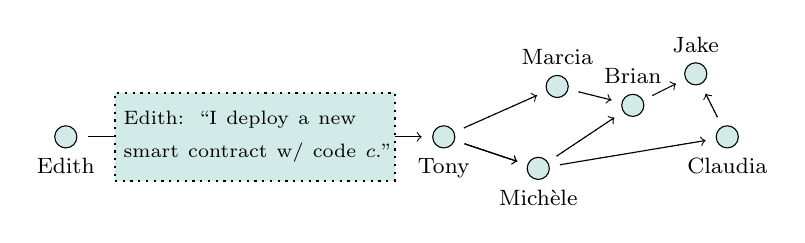
\begin{tikzpicture}[domain=-8:8, scale=0.8]

% transaction
\uncover<3->{
	\coordinate (c1) at (0,0);
	\coordinate (c2) at (6,0);
	\filldraw[draw=black,fill=highlight!50] (c1) circle (5pt) node[below=0.15cm,color=black]{\footnotesize{Edith}};
	\draw[shorten >=0.28cm,shorten <=0.28cm,->] (c1) to[] (c2);
}

% network
\uncover<2->{
\coordinate (c3) at (7.8,0.8);
\coordinate (c4) at (7.5,-0.5);
\coordinate (c5) at (9,0.5);
\coordinate (c6) at (10,1);
\coordinate (c7) at (10.5,0);
\filldraw[draw=black,fill=highlight!50] (c2) circle (5pt) node[below=0.15cm,color=black]{\footnotesize{Tony}};
\filldraw[draw=black,fill=highlight!50] (c3) circle (5pt) node[above=0.15cm,color=black]{\footnotesize{Marcia}};
\filldraw[draw=black,fill=highlight!50] (c4) circle (5pt) node[below=0.15cm,color=black]{\footnotesize{Michèle}};
\filldraw[draw=black,fill=highlight!50] (c5) circle (5pt) node[above=0.15cm,color=black]{\footnotesize{Brian}};
\filldraw[draw=black,fill=highlight!50] (c6) circle (5pt) node[above=0.15cm,color=black]{\footnotesize{Jake}};
\filldraw[draw=black,fill=highlight!50] (c7) circle (5pt) node[below=0.15cm,color=black]{\footnotesize{Claudia}};
}

\uncover<3->{
\draw[shorten >=0.28cm,shorten <=0.28cm,->] (c2) to[] (c3);
\draw[shorten >=0.28cm,shorten <=0.28cm,->] (c2) to[] (c4);
\draw[shorten >=0.28cm,shorten <=0.28cm,->] (c2) to[] (c4);
\draw[shorten >=0.28cm,shorten <=0.28cm,->] (c3) to[] (c5);
\draw[shorten >=0.28cm,shorten <=0.28cm,->] (c4) to[] (c5);
\draw[shorten >=0.28cm,shorten <=0.28cm,->] (c4) to[] (c7);
\draw[shorten >=0.28cm,shorten <=0.28cm,->] (c5) to[] (c6);
\draw[shorten >=0.28cm,shorten <=0.28cm,->] (c7) to[] (c6);
}

\uncover<2>{
\draw[shorten >=0.28cm,shorten <=0.28cm, dotted] (c2) to[] (c3);
\draw[shorten >=0.28cm,shorten <=0.28cm, dotted] (c2) to[] (c4);
\draw[shorten >=0.28cm,shorten <=0.28cm, dotted] (c2) to[] (c4);
\draw[shorten >=0.28cm,shorten <=0.28cm, dotted] (c3) to[] (c5);
\draw[shorten >=0.28cm,shorten <=0.28cm, dotted] (c4) to[] (c5);
\draw[shorten >=0.28cm,shorten <=0.28cm, dotted] (c4) to[] (c7);
\draw[shorten >=0.28cm,shorten <=0.28cm, dotted] (c5) to[] (c6);
\draw[shorten >=0.28cm,shorten <=0.28cm, dotted] (c7) to[] (c6);
}

% value transaction
\uncover<3>{
\filldraw[fill=highlight!50,dotted,thick] (0.78,-0.7) -- (5.22,-0.7) -- (5.22,0.7) -- (0.78,0.7) -- (0.78,-0.7) node[midway, right=-0.02cm,text width=4.25cm]{\scriptsize{Edith: ``I transfer one \\ Ether to Daniel.''}};
}

% smart contract interaction
\uncover<4>{
\filldraw[fill=highlight!50,dotted,thick] (0.78,-0.7) -- (5.22,-0.7) -- (5.22,0.7) -- (0.78,0.7) -- (0.78,-0.7) node[midway, right=-0.02cm,text width=4.25cm]{\scriptsize{Edith: ``Execute function \\ $f$ of \texttt{0x...} with data $d$.''}};
}

% smart contract deployment
\uncover<5>{
\filldraw[fill=highlight!50,dotted,thick] (0.78,-0.7) -- (5.22,-0.7) -- (5.22,0.7) -- (0.78,0.7) -- (0.78,-0.7) node[midway, right=-0.02cm,text width=4.25cm]{\scriptsize{Edith: ``I deploy a new \\ smart contract w/ code $c$.''}};
}


\end{tikzpicture}

	\end{figure}\vspace{1em}
}

\begin{columns}
	\begin{column}{0.5\textwidth}
	\uncover<3->{
		Transaction types:
        \begin{itemize}
		\item<3-> \alert<3>{Value transactions}
		\item<4-> \alert<4>{Smart contract interactions}
		\item<5-> \alert<5>{Smart contract deployment}
		\end{itemize}
		}
	\end{column}
	\begin{column}{0.5\textwidth}
	\uncover<2->{
	Peer-to-Peer Network:
        \begin{itemize}
		\item<1-> Permissionless
		\item<1-> Censorship-resistant
		\item<1-> No special privileges
		\end{itemize}
		}
	\end{column}
\end{columns}

\end{frame}
%%%

%%% TODO: check if this should be added in the slide deck?
%\begin{frame}{SPV, Proxy Connections and Managed Accounts}
%
%\uncover<1->{\color{focus} \textbf{Not everyone is running a full node!} \color{black}} \\ \vspace{1em}
%
%\uncover<2->{\textbf{Managed Accounts}}
%	
%	\begin{itemize}
%		\item<2-> User has no direct control over funds!
%		\item<2-> User relies on centralized party for transaction verification.
%	\end{itemize}
%
%	\vspace{1em}	
%		
%	\uncover<3->{\textbf{Proxy Connections}}
%		
%		\begin{itemize}
%		\item<3-> User relies on centralized party for transaction verification.
%	\end{itemize}		
%	
%	\vspace{1em}
%	
%	\uncover<4->{\textbf{Simple Payment Verification Clients}}
%	
%	\begin{itemize}
%		\item<4-> User relies on a set of nodes for transaction propagation and verification.
%
%	\end{itemize}
%	
%\end{frame}
%%%	

%%%
\begin{frame}{Transaction Legitimacy}
\textbf{Goal:} Ensure transaction \textcolor{focus}{authenticity} and \textcolor{focus}{integrity}, i.e., ensure that the transaction was initiated by the owner of a specific address.
\uncover<2->{
		\center
		\input{../assets/figures/transaction-legit.tex}
		}
\uncover<3->{
		\vspace{1em}
		\input{../assets/figures/transaction-manipulation.tex}
	}
\end{frame}
%%%

%%%
\begin{frame}{Public/Private Key Pair}

	\input{../assets/figures/key_creation}

\vspace{1em}

\textbf{Two key principles:}
\begin{enumerate}
\item<1-> Private key is created (chosen) without the help of an intermediary, and can be used to derive public key.
\item<2-> If information is encrypted with one key, it can only be decrypted with the other key.
\end{enumerate}

\vspace{1.5em}

\uncover<3->{
	
	\begin{columns}[T]
		\begin{column}{0.6\textwidth}
			\vspace{-1.0em}
			\begin{alertblock}{IMPORTANT!}
				\textbf{Private key must remain secret at all time. \\
				Public key can be shared freely.}
			\end{alertblock}		
		\end{column}
		
	\end{columns}
}
\end{frame}
%%%

%%%
\begin{frame}{Two Distinct Applications}
	\input{../assets/figures/publickeycrypto_applications}
\end{frame}
%%%


%%%
\begin{frame}{Verification of Transactions}
	\begin{figure}[h!]
		\center
		\input{../assets/figures/transaction-encryption.tex}
		\caption*{Encryption and decryption of the transaction message}
		\label{fig:asymmeinfach}
	\end{figure}
	
\end{frame}
%%%

%%%
\begin{frame}{Fundamentals: Cryptography}

\textbf{Prerequisites:}
\begin{columns}

	\begin{column}{0.45\textwidth}
		\begin{figure}
		\includegraphics[width = \textwidth]{../assets/images/hash_functions_video.png}
		\caption*{\href{https://www.youtube.com/watch?v=WXszGuXHFNk}{\link Hash Functions}}
		\end{figure}
	\end{column}
	\begin{column}{0.45\textwidth}
		\begin{figure}
		\includegraphics[width = \textwidth]{../assets/images/asymm_crypto_video.png}
		\caption*{\href{https://www.youtube.com/watch?v=rScMINd5S7I}{\link Asymmetric Cryptography}}
		\end{figure}
	\end{column}
	
\end{columns}

\end{frame}
%%%

%%%
\begin{frame}{Transaction Consensus}
\textbf{Goal:} Deciding which (legitimate) transactions are \textcolor{focus}{valid}. \\
\vspace{1em}
\uncover<2->{
\textbf{Potential problem:} Assume both transactions have valid signatures, but they compete with each other. What now? \\
\begin{figure}[h!]
	\center
	\input{../assets/figures/double-spend.tex}
\end{figure}
}

\uncover<3->{
\begin{alertblock}{Key insights}
Transactions modify the data structure. There needs to be a process that ensures that all network participants agree on which transactions are valid.
\end{alertblock}
}

\end{frame}
%%%

%%%
\begin{frame}{State Transitions}
	\textbf{Goal:} Deciding which (legitimate) transactions are \textcolor{focus}{valid}. \\
\vspace{1em}
\textbf{Potential problem:} Assume both transactions have valid signatures, but they compete with each other. What now? \\
\begin{figure}[h!]
	\center
	\input{../assets/figures/competing-transactions.tex}
\end{figure}

\uncover<2->{
\begin{alertblock}{Key insights}
Every transaction type modifies the data structure. Depending on the order in which the transactions are executed the current state of the ledger can be different.
\end{alertblock}
}

\end{frame}
%%%

%%%
\begin{frame}{Personal Database and Transaction Queue}
	\begin{minipage}{0.15\textwidth}
		\center
		\includegraphics[width=2.4cm]{../assets/images/miner_single.png}
	\end{minipage}
	\begin{minipage}{0.1\textwidth}
		
\begin{tikzpicture}[scale=1]
			\draw [decorate,decoration={brace,amplitude=10pt}, color = mint, line width=2pt]
			(0.5,0.0) -- (0.5,5.5) node [black,midway,xshift=-0.8cm] 
			{\footnotesize};
		\end{tikzpicture}
	\end{minipage}
	\begin{minipage}{0.7\textwidth}
		\uncover<1->{\textbf{Personal Version of the Blockchain}}
		\begin{itemize}
			\item<1-> Personal ledger of valid transactions in block structure.
			\item<1-> Has an incentive to keep in sync with consensus.
		\end{itemize}
		\vspace{1em}
		\uncover<2->{\textbf{Personal Transaction Queue}}
		\begin{itemize}
			\item<2-> Transactions that are not yet valid.
			\item<2-> Waiting for inclusion in database $\rightarrow$ queue.
		\end{itemize}
	\end{minipage}
\end{frame}
%%%

%%%
\begin{frame}{Block Creation}
	\textbf{Network participants bundle and order transactions:}
	\begin{columns}
		\begin{column}{0.45\textwidth}	
			\begin{figure}
				\includegraphics[width = \textwidth]{../assets/images/globe.png}
			\end{figure}
		\end{column}
		\begin{column}{0.45\textwidth}	
			\begin{figure}
				\includegraphics[width = \textwidth]{../assets/images/globe.png}
			\end{figure}
		\end{column}
	\end{columns}
\end{frame}
%%%

%%%
\begin{frame}{Consensus Protocols}

\begin{figure}
	\includegraphics[width = 0.5\textwidth]{../assets/images/globe.png}	
\end{figure}

\vspace{1.5em}

\begin{itemize}
	\item<2-> \textbf{Proof of Authority (PoA):} one party decides
	\item<3-> \textbf{Proof of Work (PoA):} decentralized lottery
	\item<4-> \textbf{Proof of Stake (PoS):} 

\end{itemize}

	% PoA -- trusted party decides
	% PoW -- decentralized lottery
	% PoS -- collateral that secures the network
	% Reference video "alternative consensus protocols"
\end{frame}
%%%

%%% TODO: whitepaper
\begin{frame}{Recommended Reading}
\begin{columns}
	\begin{column}{0.3\textwidth}
	\center
	\includegraphics[width=\textwidth , frame]{../assets/images/short-introduction-cryptocurrencies.png}
	\end{column}
	\begin{column}{0.7\textwidth}
	\textbf{A Short Introduction to the World of Cryptocurrencies} \\
	Aleksander Berentsen and Fabian Schär \\
	\link \href{https://files.stlouisfed.org/files/htdocs/publications/review/2018/01/10/a-short-introduction-to-the-world-of-cryptocurrencies.pdf}{Online PDF}
	\end{column}
\end{columns}
\end{frame}
%%%

%%% TODO: yellowpaper
\begin{frame}{Recommended Reading 2}
\begin{columns}
	\begin{column}{0.3\textwidth}
	\center
	\includegraphics[width=\textwidth , frame]{../assets/images/short-introduction-cryptocurrencies.png}
	\end{column}
	\begin{column}{0.7\textwidth}
	\textbf{A Short Introduction to the World of Cryptocurrencies} \\
	Aleksander Berentsen and Fabian Schär \\
	\link \href{https://files.stlouisfed.org/files/htdocs/publications/review/2018/01/10/a-short-introduction-to-the-world-of-cryptocurrencies.pdf}{Online PDF}
	\end{column}
\end{columns}
\end{frame}
%%%

%%%
%\begin{frame}%[allowframebreaks]
%\frametitle{References}
%	\bibliographystyle{amsplain}
%	\bibliography{../assets/bib/refs}
%\end{frame}
%%%

\end{document}